\documentclass[11pt,a4paper]{article}
\usepackage[margin=1in]{geometry}
\usepackage{hyperref}
\usepackage{enumitem}
\usepackage{graphicx}
\usepackage{xcolor}
\usepackage{titling}
\usepackage{tikz}
\usetikzlibrary{positioning,arrows.meta}

\makeatletter
\newcommand{\BvrSetLabInstructor}[1]{\gdef\Bvr@LabInstructor{#1}}
\newcommand{\Bvr@LabInstructor}{Dr. Raghav B. Venkataramaiyer}
\newcommand{\BvrLabInstructorValue}{\Bvr@LabInstructor}
\makeatother

\pretitle{\begin{center}\bfseries\fontsize{18bp}{18bp}\selectfont}
\makeatletter
\newcommand{\BvrSubtitle}[1]{\posttitle{\par\end{center}\begin{center}\large#1\end{center}\vskip 0.5em}}
\makeatother

\newcommand{\BvrHint}[1]{{\normalfont\normalsize\itshape\hfill #1}}

\title{CP Recall}
\BvrSetLabInstructor{Dr. Raghav B. Venkataramaiyer}

\BvrSubtitle{%
Adaptive Competitive Programming Pattern Retention System \\
Project Proposal for UCS503P \\
Submitted to: \BvrLabInstructorValue \\ \bfseries
Thapar Institute of Engineering and Technology%
}

\author{
Subham Kumar, CSED -- Roll No: 1024030665
\and
Tanush Grover, CSED -- Roll No: 1024030666
\and
Shubhi Singh, CSED -- Roll No: 1024030669
}
\date{August 2026}

\begin{document}
\maketitle

\section{Higher-Order Goal}
This project aims to make DSA/competitive-programming practice more effective by helping students retain reusable problem-solving patterns instead of only accumulating a count of solved questions. The immediate engineering goal is narrower: build a practical system that tracks a student's performance at the pattern level and schedules meaningful reviews using new problems from the same pattern family.

\section{Time-to-Value}
\begin{itemize}[leftmargin=0.7cm]
\item The first working iteration should demonstrate the core loop end to end --- problem $\rightarrow$ pattern $\rightarrow$ performance $\rightarrow$ mastery $\rightarrow$ review scheduling --- even if the surrounding parts (extension polish, analytics, UI) are minimal.
\item Later iterations can improve extension integration, problem-selection logic, dashboards, and usability.
\item Success for the first iteration is a working pipeline for a small, curated set of patterns and problems, not full coverage of LeetCode.
\end{itemize}

\section{Problem Statement}
\begin{itemize}[leftmargin=0.7cm]
\item A solved-problem count does not tell a student whether they can apply the underlying technique to a new problem --- students often remember the specific solution, not the pattern.
\item Existing platforms do not give a simple, pattern-level view of which DSA patterns a student is actually strong or weak in.
\item Students generally do not know which patterns are due for revision, and manually tracking this for many patterns is tedious.
\item Re-solving the exact same problem is a weak test of retention, since the student may just remember the earlier solution.
\item There is a need for a lightweight companion tool that tracks pattern-level performance, schedules reviews, and tests retention using a different, suitable problem from the same pattern family.
\end{itemize}

\section{Proposed Solution}
\subsection{Overview}
CP Recall is a browser extension paired with a backend application. The extension works alongside LeetCode and shows a contextual Revision Assistant when relevant to the problem currently open. The backend tracks problems, patterns, performance history, pattern-level mastery, and the review schedule. Main components:
\begin{itemize}[leftmargin=0.7cm]
\item \textbf{LeetCode browser extension:} problem detection + contextual Revision Assistant
\item \textbf{Problem-pattern mapping:} initially curated manually, e.g. 3Sum $\rightarrow$ Two Pointers
\item \textbf{Performance tracking:} per attempt and pattern-level mastery tracking
\item \textbf{FSRS-based review scheduling and same-pattern problem selection}
\item \textbf{Problem Library, Home Dashboard, Pattern Dashboard, Problem Details:} review information appears inside these views; there is no separate revision screen
\item \textbf{Review/performance history storage}
\end{itemize}

\subsection{Core Workflow}

\begin{center}
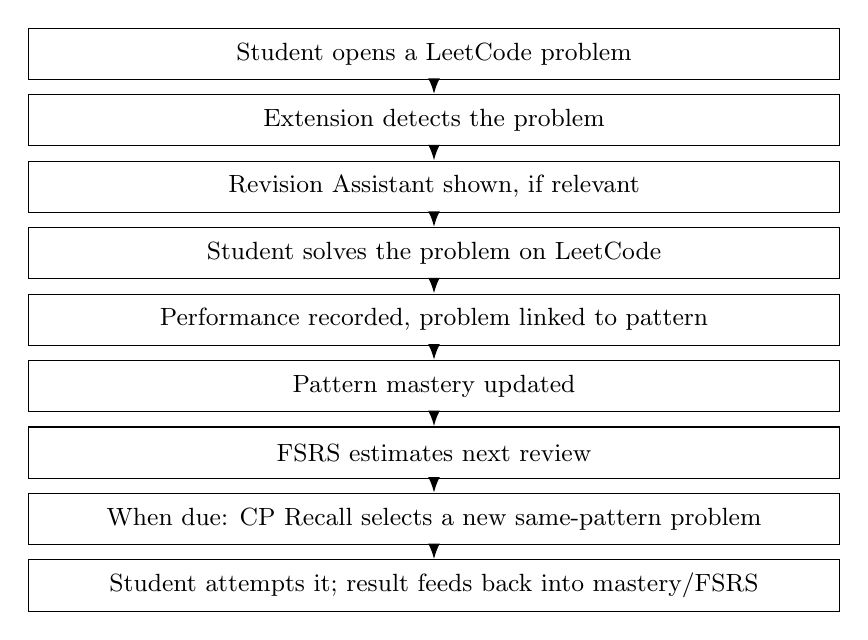
\begin{tikzpicture}[
    box/.style={
        draw,
        rectangle,
        minimum width=0.85\textwidth,
        minimum height=0.65cm,
        align=center,
        font=\small
    },
    arrow/.style={
        -{Latex[length=2mm]},
        thick
    },
    node distance=0.18cm
]

\node[box] (a) {Student opens a LeetCode problem};
\node[box, below=of a] (b) {Extension detects the problem};
\node[box, below=of b] (c) {Revision Assistant shown, if relevant};
\node[box, below=of c] (d) {Student solves the problem on LeetCode};
\node[box, below=of d] (e) {Performance recorded, problem linked to pattern};
\node[box, below=of e] (f) {Pattern mastery updated};
\node[box, below=of f] (g) {FSRS estimates next review};
\node[box, below=of g] (h) {When due: CP Recall selects a new same-pattern problem};
\node[box, below=of h] (i) {Student attempts it; result feeds back into mastery/FSRS};

\draw[arrow] (a) -- (b);
\draw[arrow] (b) -- (c);
\draw[arrow] (c) -- (d);
\draw[arrow] (d) -- (e);
\draw[arrow] (e) -- (f);
\draw[arrow] (f) -- (g);
\draw[arrow] (g) -- (h);
\draw[arrow] (h) -- (i);

\end{tikzpicture}
\end{center}

FSRS decides when a pattern is due; CP Recall's own selection logic decides which new problem to give for that review. We are keeping these as two separate modules.
FSRS decides when a pattern is due; CP Recall's own selection logic decides which new problem to give for that review. We are keeping these as two separate modules.

FSRS decides when a pattern is due; CP Recall's own selection logic decides which new problem to give for that review. We are keeping these as two separate modules.

\section{Operational Constraints}
\begin{itemize}[leftmargin=0.7cm]
\item \textbf{Semester timeline:} scope has to fit what a 3-person team can build in one term.
\item \textbf{LeetCode dependency:} the extension depends on LeetCode's current page structure and may need updates if that changes.
\item \textbf{Curated dataset:} the initial problem-pattern dataset will be small and manually curated, not auto-generated.
\item \textbf{Code analysis limitation:} no automatic understanding of arbitrary submitted code --- only practical, observable signals are recorded.
\item \textbf{FSRS dependency:} FSRS is an external component; we are integrating it, not building our own scheduler.
\item \textbf{Pilot size:} pilot testing will involve a small group of student users, not a large user base.
\item \textbf{Feature scope:} we are avoiding unnecessary features and keeping the system lightweight.
\end{itemize}

\section{Solution Approach}
This is a Software Engineering project, so the focus is on workflow, modular design, and data handling rather than research. Key modules:

\subsection{LeetCode Browser Extension}
Detects the currently open problem and shows the Revision Assistant only when relevant --- not as a permanent sidebar. The student still solves the problem on LeetCode itself; the extension is a thin assisting layer.

\subsection{Pattern Identification and Tracking}
Each problem is linked to one or more patterns using a manually curated mapping to start with, which can be extended over time.

\subsection{Performance Review}
After an attempt, we record signals such as time taken, number of submissions, final result, approximate efficiency/time complexity where reasonably available, and hints used --- not a full analysis of the submitted code.

\subsection{Pattern Mastery}
Attempt-level performance is aggregated into a per-pattern mastery indicator (roughly a percentage). This is an evolving indicator, not an exact measurement.

\subsection{FSRS-Based Scheduling}
FSRS (Free Spaced Repetition Scheduler) is used to estimate a reasonable interval before the next review, based on past performance on that pattern. FSRS answers: ``when should this pattern be reviewed?''

\subsection{Problem Selection for Review}
When a pattern is due, CP Recall's own logic picks a different, suitable problem from the same pattern family (initial rule: unattempted or less-recently-attempted, similar/slightly higher difficulty). This answers: ``which new problem from this pattern should be used?''

\section{Web Architecture}
\begin{center}
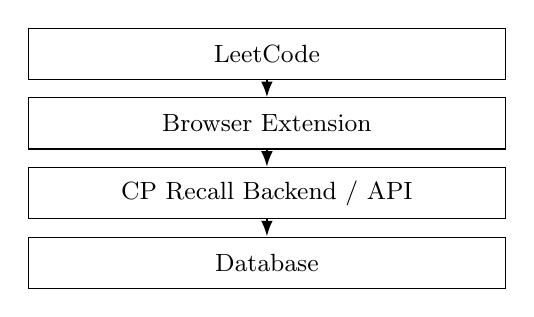
\begin{tikzpicture}[box/.style={draw,rectangle,minimum width=0.5\textwidth,minimum height=0.65cm,align=center,font=\small},arrow/.style={-{Latex[length=2mm]},thick},node distance=0.22cm]
\node[box] (a) {LeetCode};
\node[box,below=of a] (b) {Browser Extension};
\node[box,below=of b] (c) {CP Recall Backend / API};
\node[box,below=of c] (d) {Database};
\draw[arrow] (a)--(b); \draw[arrow] (b)--(c); \draw[arrow] (c)--(d);
\end{tikzpicture}
\end{center}
\begin{itemize}[leftmargin=0.7cm]
\item \textbf{Frontend:} Home Dashboard, Pattern Dashboard, Problem Library, Problem Details.
\item \textbf{Backend/API:} authentication, problem/pattern management, performance tracking, pattern mastery, FSRS scheduling, review/problem selection, dashboard data.
\item \textbf{Database:} users, problems, patterns, problem-pattern links, attempts, mastery, review history.
\item \textbf{Extension:} thin layer that talks to the backend API; does not hold business logic of its own.
\end{itemize}
The exact technology stack will be finalized during implementation based on project requirements; we intend to keep frontend, backend, and extension loosely coupled so each can be built and tested independently.

\section{CI/CD and Fast Delivery}
\begin{itemize}[leftmargin=0.7cm]
\item Automated build and test run on every change.
\item Backend unit tests and basic linting as part of the pipeline.
\item Repeatable deployment to a staging environment.
\item Incremental feature releases instead of one large release at the end.
\end{itemize}
None of this is implemented yet at the proposal stage --- this is what we plan to set up alongside development.

\section{Evaluation Criteria}
\subsection{Primary Evaluation Metric}
\textbf{Pattern Retention Success Rate} --- the percentage of due-review attempts in which the student successfully solves the new (same-pattern) problem given by CP Recall.
\begin{itemize}[leftmargin=0.7cm]
\item \textbf{Measured as:} (successful new-problem attempts at review) $\div$ (total due-review attempts), using recorded attempt outcomes.
\item This is the primary metric because it directly checks whether the core idea --- testing retention with a different problem --- is working.
\item \textbf{Proposed target (not an achieved result):} a reasonable success rate during the pilot window, to be refined once we have initial data.
\end{itemize}

\subsection{Secondary Evaluation Metrics}
\begin{itemize}[leftmargin=0.7cm]
\item \textbf{Review adherence} --- how often due reviews are actually attempted.
\item \textbf{Mastery progression} --- whether pattern mastery trends upward over repeated attempts.
\item \textbf{Review scheduling usefulness} --- whether FSRS-based intervals feel practical to students.
\item \textbf{Problem-selection usefulness} --- whether the new problem given for review feels like a fair test of the pattern.
\item \textbf{User usability} --- feedback on the dashboards and overall workflow.
\end{itemize}

\subsection{Pilot Validation Plan}
\begin{itemize}[leftmargin=0.7cm]
\item Recruit a small group of student users (classmates/volunteers) to use CP Recall for a few weeks.
\item Log performance and review outcomes as they solve and revisit problems.
\item Compare retention across review attempts and collect usability feedback via a short questionnaire.
\item Given the small sample size and short duration, results will be indicative rather than conclusive.
\end{itemize}

\section{Scalability}
\begin{itemize}[leftmargin=0.7cm]
\item Frontend and backend kept decoupled.
\item Indexed queries for problems/patterns, especially for Problem Library filtering.
\item Pagination in the Problem Library instead of loading everything at once.
\item Largely stateless API design where practical.
\item Ability to add more patterns/problems without structural changes.
\item FSRS scheduling kept as its own module so it can be optimized independently.
\item Extension and backend kept separate so either can evolve without breaking the other.
\item The pattern-tracking + FSRS-review model is not tied to DSA/LeetCode specifically --- the same problem-pattern-mastery-review structure could later extend to other practice domains such as UI/frontend practice questions or cybersecurity practice challenges, by swapping the problem source and pattern set.
\end{itemize}

\section{Engine Availability Heuristic}
The core ``engine'' our project depends on --- FSRS --- is already a mature, open-source scheduling algorithm with existing library implementations, so we do not need to design or tune a spaced-repetition algorithm ourselves. We only need to integrate it and feed it the performance data our system records.

Beyond FSRS, mature ready-to-use components exist for the rest of the stack too --- web frontend frameworks, backend/REST frameworks, relational or document databases, browser-extension APIs, authentication approaches, test frameworks, and CI/CD tooling. We plan to use these established components and put our effort into the parts that are actually specific to CP Recall: the problem-pattern data model, mastery aggregation, and same-pattern problem-selection logic around the FSRS engine.

\section{Project Scope and Deliverables}
\subsection{Initial Deliverable}
\begin{itemize}[leftmargin=0.7cm]
\item User authentication
\item Problem and pattern data management (curated dataset)
\item Basic browser extension prototype for LeetCode
\item Contextual Revision Assistant
\item Performance recording after an attempt
\item Pattern mastery tracking
\item FSRS integration for review scheduling
\item Home Dashboard, Pattern Dashboard, Problem Library, Problem Details
\item Basic testing of the above modules
\end{itemize}

\subsection{Subsequent Deliverables}
\begin{itemize}[leftmargin=0.7cm]
\item Improved problem-selection logic
\item Richer analytics on the dashboards
\item Improved browser-extension integration and edge-case handling
\item Additional pattern categories in the dataset
\item Usability improvements based on pilot feedback
\end{itemize}

\section{Risks and Mitigations}
\begin{itemize}[leftmargin=0.7cm]
\item \textbf{Browser extension limitations / LeetCode page changes} --- keep extension logic modular and separated from CP Recall's own application logic.
\item \textbf{Problem-pattern mapping quality} --- start with a small, manually validated mapping and expand gradually.
\item \textbf{Mastery estimation limitations} --- treat mastery as an evolving indicator, not an absolute measure.
\item \textbf{FSRS integration complexity} --- wrap FSRS behind a well-defined internal module and test it independently.
\item \textbf{User adoption} --- keep the workflow simple and avoid unnecessary manual data entry.
\item \textbf{Evaluation limitations} --- use a small controlled pilot group with clearly defined metrics (Section 9).
\end{itemize}

\section{Summary}
CP Recall tracks DSA/competitive-programming mastery at the pattern level instead of just counting solved problems, uses FSRS to decide when a pattern is due for review, and tests that review with a new problem from the same pattern family rather than the original question. As a Software Engineering project, our focus is on getting the workflow, data model, and module boundaries right, and delivering a working initial version (Section 12.1) before attempting later improvements. We revise the pattern, not the question.

\end{document}
